\section{Second-Order Partial Derivatives} \label{S:10.3.Second_Order_Partial_Derivatives}

\vspace*{-14 pt}
\framebox{\hspace*{3 pt}
  \parbox{6.25 in}{
    \begin{goals} 
    \item Given a function $f$ of two independent
      variables $x$ and $y$, how are the second-order
      partial derivatives of $f$ defined?  
    \item What do the second-order
      partial derivatives $f_{xx}$, $f_{yy}$, $f_{xy}$, and $f_{yx}$
      of a function $f$ tell us about the function's behavior?
%  \item What special relationship exists among the second-order mixed partial
 %   derivatives $f_{xy}$ and $f_{yx}$ for a function $f$ of two variables?
\end{goals}} \hspace*{3 pt}}

\subsection*{Introduction}

Recall that for a single-variable function $f$, the second derivative of $f$ is defined to be the derivative of the first derivative.  That is, $f''(x) = \frac{d}{dx}[f'(x)]$, which can be stated in terms of the limit definition of the derivative by writing
$$f''(x) = \lim_{h \to 0} \frac{f'(x+h) - f'(x)}{h}.$$
%The second derivative measures the instantaneous rate of change of the first derivative, and thus the instantaneous rate of change of the slope of the tangent line to the function $f$.  Because of this relationship, we know that the second derivative is directly connected to the concavity of the function:  $f$ is concave up if and only if $f''$ is positive, and $f$ is concave down if and only if $f''$ is negative.  
In what follows, we begin exploring the four different second-order partial derivatives of a function of two variables and seek to understand what these various derivatives tell us about the function's behavior.

\begin{pa} \label{PA:10.3} Once again, let's consider the function $f$ defined by $ f(x,y) = \frac{x^2\sin(2y)}{32}$ 
  \begin{figure}[ht]
    \begin{center}
      \includegraphics{figures/fig_10_2_trace_x_a.eps}
      \hspace*{20pt}
      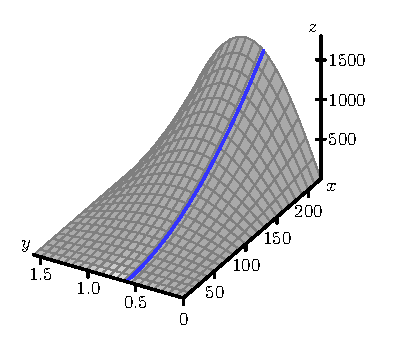
\includegraphics{figures/fig_10_2_trace_y_a.eps}
    \end{center}
    \caption{The range function with traces $y=0.6$ and $x=150$.}
    \label{F:10.3.preview}
  \end{figure}
that measures a projectile's range as a function of its
  initial speed $x$ and launch angle $y$.  The graph of this function,
  including traces with $x=150$ and $y=0.6$, is shown in Figure
  \ref{F:10.3.preview}. 

  \ba
  \item Compute the partial derivative $f_x$ and notice that $f_x$ itself is a
    new function of $x$ and $y$.
  \item We may now compute the partial derivatives of $f_x$.  Find the
    partial derivative $f_{xx} = (f_x)_x$ and evaluate $f_{xx}(150,
    0.6)$.  

  \item Figure \ref{F:10.3.preview.xx} shows the trace of $f$ with
    $y=0.6$ with three tangent lines included.  Explain how your
    result from part (b) of this preview activity is reflected in
    this figure.  

  \begin{figure}[ht]
    \begin{center}
      \scalebox{0.8}{\includegraphics{figures/fig_10_3_preview_xx.eps}}
    \end{center}
    \caption{The trace with $y=0.6$.}
    \label{F:10.3.preview.xx}
  \end{figure}

%\item Still considering $f_x$, compute its other partial derivative,
%  $f_{xy} = (f_x)_y$, and evaluate $f_{xy}(150, 0.6)$.
  
%  \item Figure \ref{F:10.3.preview.xy} shows the traces $f(x,b)$ with
 %   $b=0.4$, $b=0.6$, and $b=0.8$ with tangent lines at $x=150$
 %   included.  Explain how your 
 %   result from the previous part of this activity is reflected in
 %   this figure.  

%  \begin{figure}[ht]
%    \begin{center}
%      \scalebox{0.8}{\includegraphics{figures/fig_10_3_preview_yx.eps}}
%    \end{center}
%    \caption{The traces with $y=0.4$, $y=0.6$ and $y=0.8$.}
%    \label{F:10.3.preview.xy}
%  \end{figure}

  \item Determine the partial derivative $f_y$, and then find the partial
    derivative $f_{yy}=(f_y)_y$.  Evaluate $f_{yy}(150, 0.6)$.

%  \item The left side of Figure \ref{F:10.3.preview.y} shows traces
%    $f(a, y)$ with $a=125$, $a=150$, and $a=175$.  Explain how the
%    value of $f_{yx}(150,0.6)$ is reflected in this figure.  

  \begin{figure}[ht]
    \begin{center}
%      \includegraphics{figures/fig_10_3_preview_xy.eps}
%      \hspace*{20pt}
      \includegraphics{figures/fig_10_3_preview_yy.eps}
    \end{center}
    \caption{More traces of the range function.}
    \label{F:10.3.preview.y}
  \end{figure}

  \item Figure \ref{F:10.3.preview.y} shows the
    trace $f(150, y)$ and includes three tangent lines.
    Explain how the value of $f_{yy}(150,0.6)$ is reflected in this figure.  

%  \item What do you notice about the relationship between $f_{xy}$ and
%    $f_{yx}$?  

  \item Because $f_x$ and $f_y$ are each functions of both $x$ and $y$, they each have two partial derivatives.  Not only can we compute $f_{xx} = (f_x)_x$, but also $f_{xy} = (f_x)_y$; likewise, in addition to $f_{yy} = (f_y)_y$, but also $f_{yx} = (f_y)_x$.  For the range function $f(x,y) = \frac{x^2\sin(2y)}{32}$, use your earlier computations of $f_x$ and $f_y$ to now determine $f_{xy}$ and $f_{yx}$.  Write one sentence to explain how you calculated these ``mixed'' partial derivatives.

    \ea


\end{pa} 

\begin{activitySolution} 
  \ba
  \item The partial derivative $f_x$ is given by
    \[f_x(x,y) = \frac{2x\sin(2y)}{32} = \frac{x\sin(2y)}{16}.\]
 
  \item Differentiating $f_x$ with respect to $x$ yields
\[f_{xx}(x,y) = (f_x)_x(x,y) = \frac{\sin(2y)}{16}.\]
So $f_{xx}(150,0.6) = \frac{1}{16} \sin(1.2) \approx 0.058$. 

  \item The partial derivative $f_{xx} = (f_x)_x$ tells us how $f_x$ changes as we increase $x$ while $y$ remains constant. Now $f_x$ represents the slope of the tangent line to the trace of $f$ in the $x$ direction, so the fact that $f_{xx}(150,0.6) \approx 0.058$ tells us that the slopes of the tangent lines to the trace of $f$ in the $x$-direction are increasing by approximately 0.058 for every one unit increase in $x$ from $150$ if $y$ remains constant at $0.06$. This is reflected in the small increases in the slopes of the tangent lines as $x$ increases in the figure.  

  \item The partial derivative $f_y$ is given by
    \[f_y(x,y) = \frac{2x^2\cos(2y)}{32} = \frac{x^2\cos(2y)}{16}.\]
 Differentiating $f_y$ with respect to $y$ yields
\[f_{yy}(x,y) = (f_y)_y(x,y) = \frac{-2x^2\sin(2y)}{16} = -\frac{x^2\sin(2y)}{8}.\]
So $f_{yy}(150,0.6) = -\frac{150^2}{8} \sin(1.2) \approx -2621.36$. 


  \item The partial derivative $f_{yy} = (f_y)_y$ tells us how $f_y$ changes as we increase $y$ while $x$ remains constant. Now $f_y$ represents the slope of the tangent line to the trace of $f$ in the $y$ direction, so the fact that $f_{yy}(150,0.6) \approx -2621.36$ tells us that the slopes of the tangent lines to the trace of $f$ in the $y$-direction are decreasing by approximately 2621.26 for every one unit increase in $y$ from $0.6$ if $x$ remains constant at $150$. This is reflected in slopes in the figure decreasing from positive to negative. 

  \item If we treat $x$ as constant in $f_x$ and differentiate with respect to $y$ we obtain
\[f_{xy}(x,y) = (f_x)_y(x,y) = \frac{2x\cos(2y)}{16} = \frac{x\cos(2y)}{8}.\]
Similarly, if we treat $y$ as constant in $f_y$ and differentiate with respect to $x$ we obtain
\[f_{yx}(x,y) = (f_y)_x(x,y) = \frac{2x\cos(2y)}{16} = \frac{x\cos(2y)}{8}.\]
It is interesting to note that $f_{xy}(x,y) = f_{yx}(x,y)$. 

    \ea
\end{activitySolution}
\afterpa 


\subsection*{Second-order Partial Derivatives}

A function $f$ of two independent variables $x$ and $y$ has two first
order partial derivatives, $f_x$ and $f_y$. As we saw in Preview
Activity \ref{PA:10.3}, each of these first-order partial derivatives
has two partial derivatives, giving a total of four {\em second-order} partial derivatives\index{partial derivatives!second-order}:
\begin{itemize}
\item $f_{xx} = (f_x)_x = \frac{\partial}{\partial x} 
  \left(\frac{\partial
    f}{\partial x}\right) = 
  \frac{\partial^2 f}{\partial x^2}$,
\item $f_{yy} = (f_y)_y=\frac{\partial}{\partial y} 
  \left(\frac{\partial
    f}{\partial y}\right) = 
  \frac{\partial^2 f}{\partial y^2}$,
\item $f_{xy} = (f_x)_y=\frac{\partial}{\partial y} 
  \left(\frac{\partial
    f}{\partial x}\right) = 
  \frac{\partial^2 f}{\partial y \partial x}$,
\item $f_{yx}=(f_y)_x=\frac{\partial}{\partial x} 
  \left(\frac{\partial
    f}{\partial y}\right) = 
  \frac{\partial^2 f}{\partial x \partial y}$.
\end{itemize}

The first two are called \emph{unmixed} second-order partial
derivatives\index{partial derivatives!second-order, unmixed} while the
last two are called the \emph{mixed} second-order partial
derivatives\index{partial derivatives!second-order, mixed}.

One aspect of this notation can be a little confusing.  The notation
$$
\frac{\partial^2 f}{\partial y\partial x} = \frac{\partial}{\partial
  y}\left(\frac{\partial f}{\partial x}\right)
$$
means that we first differentiate with respect to $x$ and then with
respect to $y$; this can be expressed in the alternate notation $f_{xy} = (f_x)_y$.  However, to find the second partial derivative
$$
f_{yx} = (f_y)_x
$$
we first differentiate with respect to $y$ and then $x$.  This means
that
$$
\frac{\partial^2 f}{\partial y\partial x} = f_{xy}, 
\hspace*{20pt}
\mbox{and}
\hspace*{20pt}
\frac{\partial^2 f}{\partial x\partial y} = f_{yx}.
$$
Be sure to note carefully the difference between Leibniz notation and subscript notation and the order in which $x$ and $y$ appear in each.  In addition, remember that anytime we compute a partial derivative, we hold constant the variable(s) other than the one we are differentiating with respect to.

\begin{activity} \label{A:10.3.1} Find all second order partial
  derivatives of the following functions.   For each partial derivative you calculate, state explicitly which variable is being held constant.
  \ba
\item $f(x,y) = x^2y^3$
\item $f(x,y) = y\cos(x)$
\item $g(s,t) = st^3 + s^4$
\item How many second order partial derivatives does the
  function $h$ defined by $h(x,y,z) = 9x^9z-xyz^9 + 9$ have?  Find $h_{xz}$ and
  $h_{zx}$.  
  \ea

\end{activity}
\begin{smallhint}

\end{smallhint}
\begin{bighint}

\end{bighint}
\begin{activitySolution}
	\ba
	\item To begin, we calculate the first order partials, holding $y$ constant to calculate $f_x$ and $x$ constant to calculate $f_y$:
\begin{align*}
f_x(x,y) &= 2xy^3 \\
f_y(x,y) &= 3x^2y^2.
\end{align*}
The second order partial derivatives are partial derivatives of the
first order partial derivatives: 
\begin{align*}
f_{xx}(x,y) &= (f_x)_x(x,y) = 2y^3 \\
f_{xy}(x,y) &= (f_x)_y(x,y) = 6xy^2 \\
f_{yx}(x,y) &= (f_y)_x(x,y) = 6xy^2 \\
f_{yy}(x,y) &= (f_y)_y(x,y) = 6x^2y.
\end{align*}	
		
	\item To begin, we calculate the first order partials:
\begin{align*}
f_x(x,y) &= -y\sin(x) \\
f_y(x,y) &= \cos(x).
\end{align*}
The second order partial derivatives are partial derivatives of the first order partial derivatives:
\begin{align*}
f_{xx}(x,y) &= (f_x)_x(x,y) = -y\cos(x) \\
f_{xy}(x,y) &= (f_x)_y(x,y) = -\sin(x) \\
f_{yx}(x,y) &= (f_y)_x(x,y) = -\sin(x) \\
f_{yy}(x,y) &= (f_y)_y(x,y) = 0.
\end{align*}	
	
	\item To begin, we calculate the first order partials, holding $t$ constant to calculate $g_s$ and $s$ constant to calculate $g_t$:
\begin{align*}
g_s(s,t) &= t^3+4s^3 \\
g_t(s,t) &= 3st^2.
\end{align*}
The second order partial derivatives are partial derivatives of the first order partial derivatives:
\begin{align*}
g_{ss}(s,t) &= (g_s)_s(s,t) = 12s^2 \\
g_{st}(s,t) &= (g_s)_t(s,t) = 3t^2 \\
g_{ts}(s,t) &= (g_t)_s(s,t) = 3t^2 \\
g_{tt}(s,t) &= (g_t)_t(s,t) = 6st.
\end{align*}	

	
	\ea
\end{activitySolution}
\aftera


In Preview Activity \ref{PA:10.3} and Activity \ref{A:10.3.1}, you may have noticed 
that the mixed second-order partial derivatives are equal.
This observation holds generally and is known as Clairaut's Theorem.

\vspace*{5pt}
\nin 
\framebox{
  \hspace*{3 pt}
  \parbox{6.25 in}{
    \textbf{Clairaut's Theorem.} Let $f$ be a function of two variables for which
    the partial derivatives $f_{xy}$ and $f_{yx}$ are continuous near
    the point $(a,b)$.  Then
    \[f_{xy}(a,b) = f_{yx}(a,b).\]
  } 
  \hspace*{3 pt}
}
\vspace*{5pt}


\subsection*{Interpreting the second-order Partial Derivatives}

Recall from single variable calculus that the second derivative
measures the instantaneous rate of change of the derivative.  This observation is
the key to understanding the meaning of the second-order partial
derivatives.  

\begin{figure}[ht]
  \begin{center}
    \includegraphics[scale=0.8]{figures/fig_10_3_fxx_1.eps}
    \includegraphics[scale=0.8]{figures/fig_10_3_fxx_2.eps}
    \includegraphics[scale=0.8]{figures/fig_10_3_fxx_3.eps}
  \end{center}
  \caption{The tangent lines to a trace with increasing $x$.}
  \label{F:10.3.fxx}
\end{figure}

Furthermore, we remember that the second derivative of a function at a
point provides us with information about the concavity of the function
at that point.  Since the unmixed second-order partial derivative
$f_{xx}$ requires us to hold $y$ constant and differentiate twice with
respect to $x$, we may simply view $f_{xx}$ as the second derivative
of a trace of $f$ where $y$ is fixed.  As such, $f_{xx}$ will measure
the concavity of this trace.

Consider, for example, $f(x,y) = \sin(x) e^{-y}$.  Figure
\ref{F:10.3.fxx} shows the graph of this function along with the
trace given by $y=-1.5$.  Also shown are three tangent lines to this
trace, with increasing $x$-values from left to right among the three plots in Figure
\ref{F:10.3.fxx}.


That the slope of the tangent line is decreasing as $x$ increases is
reflected, as it is in one-variable calculus, in the fact that the
trace is concave down.  Indeed, we see that $f_x(x,y)=\cos(x)e^{-y}$ and so
$f_{xx}(x,y)=-\sin(x)e^{-y} < 0$, since $e^{-y} > 0$ for all values of $y$, including $y = -1.5$.

In the following activity, we further explore what second-order partial derivatives tell us about the geometric behavior of a surface.

\begin{activity} \label{A:10.3.2a} 
We continue to consider the function $f$ defined by $f(x,y) = \sin(x) e^{-y}$.
    \ba
	\item  In Figure~\ref{F:10.3.fyy}, we see the trace of $f(x,y) = \sin(x) e^{-y}$ that has $x$ held constant with $x = 1.75$. 
\begin{figure}[ht]
  \begin{center}
    \includegraphics[scale=0.8]{figures/fig_10_3_fyy_1.eps}
    \includegraphics[scale=0.8]{figures/fig_10_3_fyy_2.eps}
    \includegraphics[scale=0.8]{figures/fig_10_3_fyy_3.eps}
  \end{center}
  \caption{The tangent lines to a trace with increasing $y$.}
  \label{F:10.3.fyy}
\end{figure}
Write a couple of sentences that describe whether the slope of the tangent lines to this curve increase or decrease as $y$ increases, and, after computing $f_{yy}(x,y)$, explain how this observation is related to the value of $f_{yy}(1.75,y)$.  Be sure to address the notion of concavity in your response.

	\item  In Figure~\ref{F:10.3.fxy}, we start to think about the mixed partial derivative, $f_{xy}$.  Here, we first hold $y$ constant to generate the first-order partial derivative $f_x$, and then we hold $x$ constant to compute $f_{xy}$.  This leads to first thinking about a trace with $x$ being constant, followed by slopes of tangent lines in the $y$-direction that slide along the original trace.  You might think of sliding your pencil down the trace with $x$ constant in a way that its slope indicates $(f_x)_y$ in order to further animate the three snapshots shown in the figure.
\begin{figure}[ht]
  \begin{center}
    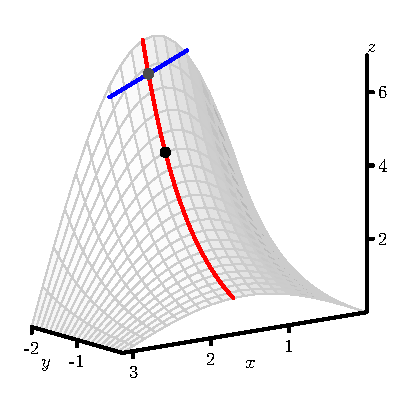
\includegraphics[scale=0.8]{figures/fig_10_3_fxy_1.eps}
    \includegraphics[scale=0.8]{figures/fig_10_3_fxy_2.eps}
    \includegraphics[scale=0.8]{figures/fig_10_3_fxy_3.eps}
  \end{center}
  \caption{The trace of $z = f(x,y) = \sin(x)e^{-y}$ with $x = 1.75$, along with tangent lines in the $y$-direction at three different points.}
  \label{F:10.3.fxy}
\end{figure}	
Based on Figure~\ref{F:10.3.fxy}, is $f_{xy}(1.75, -1.5)$ positive or negative?  Why?

	\item Determine the formula for $f_{xy}(x,y)$, and hence evaluate $f_{xy}(1.75, -1.5)$.  How does this value compare with your observations in (b)?
	
	\item We know that $f_{xx}(1.75, -1.5)$ measures the concavity of the $y = -1.5$ trace, and that $f_{yy}(1.75, -1.5)$ measures the concavity of the $x = 1.75$ trace.  What do you think $f_{xy}(1.75, -1.5)$ measures?
	
	\item On Figure~\ref{F:10.3.fxy}, sketch the trace with $y = -1.5$, and sketch three tangent lines whose slopes correspond to the value of $f_{yx}(x,-1.5)$ for three different values of $x$, the middle of which is $x = -1.5$.  Is $f_{yx}(1.75, -1.5)$ positive or negative?  Why?  What does $f_{yx}(1.75, -1.5)$ measure?


  \ea

\end{activity}
\begin{smallhint}

\end{smallhint}
\begin{bighint}

\end{bighint}
\begin{activitySolution}
\ba
\item The figures seem to indicate that the slopes of the tangent lines to the trace $f(1.75,y)$ increase as $y$ increases. Note that $\frac{d}{dy} f(1.75,y) = \frac{d}{dy} \sin(1.75) e^{-y} = -\sin(1.75) e^{-y}$, so as $y$ increases the slopes of the tangent lines become less negative. Note also that $\frac{d^2}{dy^2} f(1.75,y) = \sin(1.75)e^{-y}$ which is a decreasing function. This tells us that the $x=1.75$ trace is concave down. That means that the slopes of the tangent lines to the trace are increasing, but at a decreasing rate. This is reflected in the fact that the surface seems to be leveling off as $y$ increases. 

\item Based on the figure, the slopes of the tangent lines in the $x$ direction along the $x=1.75$ trace appear to be negative, but getting less negative as $y$ increases. So we expect $f_{xy}(1.75,-1.5)$ to be positive.  

\item Since $f_x(x,y) = \cos(x)e^{-y}$, we have $f_{xy} = -\cos(x)e^{-y}$. So $f_{xy}(1.75,-1.5) \approx 0.8$. This number is positive, as we discussed in the previous part. 

\item The quantity $f_{xy}(1.75,-1.5)$ tells us how much the slopes of the $x=1.75$ trace change as we increase $y$ from $-1.5$. Geometrically, we could describe $f_{xy}(1.75,-1.5)$ as telling us how much the surface ``twists" in the $y$ direction when $y=-1.5$ as we move along the $x=1.75$ trace. 

\item The sketches are shown below. Since $f_y(x,y) = -\sin(x)e^{-y}$, when $x$ exceeds $\frac{\pi}{2}$ and increases, $f_y(x,y)$ increases for fixed $y$. So we should expect $f_{yx}(1.75,-1.5)$ to be positive. In fact, $f_{yx}(1.75,-1.5) = 0.8$. The value of $f_{yx}(1.75,-1.5)$ measures how much the surface ``twists" in the $x$ direction when $x=1.75$ as we move along the $y=-1.5$ trace.  

   \begin{center}
      \resizebox{!}{2.0in}{\includegraphics{figures/fig_10_3_Act_2a_fyx_1.png}} \ \ \resizebox{!}{2.0in}{\includegraphics{figures/fig_10_3_Act_2a_fyx_2.png}} \ \ \resizebox{!}{2.0in}{\includegraphics{figures/fig_10_3_Act_2a_fyx_3.png}}
    \end{center}
\ea
\end{activitySolution}
\aftera


%Similarly, $f_{yy}=(f_y)_y$ tells us the instantaneous rate at which $f_y$ changes
%as we move along a trace with fixed $x$.  As such, its sign determines
%the concavity of this trace.  In our example, $f_y(x,y)=-\sin(x)e^{-y}$, so
%that $f_{yy}(x,y)=\sin(x)e^{-y}$.  Considering the trace with $x = \frac{\pi}{2}$, since $\sin(\pi/2) = 1$, it follows
%that $f_{yy}(\pi/2,y) = e^{-y} > 0$.  This fact is reflected in Figure
%\ref{F:10.3.fyy}, which shows that the slope of the tangent lines
%increase along the trace with $x = \frac{\pi}{2}$, and hence this trace is concave
%up. 

%The mixed partials, $f_{xy}$ and $f_{yx}$, require more
%thought.  Once again, recall that $f_{xy} = (f_x)_y$ measures the instantaneous rate
%of change of $f_x$ as we increase $y$.  In addition, $f_x$ measures the slope
%of the tangent line to a trace with $y$ fixed. Figure \ref{F:10.3.fxy}
%shows three such tangent lines drawn as $y$ increases.  Notice that the
%slope of the tangent lines decreases, and thus we expect that $f_{xy} <
%0$.  Indeed, $f_{xy} = -\cos(x)e^{-y} > 0$ at the point shown in the figure.  

Just as with the first-order partial derivatives, we can
approximate second-order partial derivatives in the situation where we have only
partial information about the function.

\begin{activity} \label{A:10.3.6}  As we saw in Activity
  \ref{A:10.2.12}, the wind chill $w(v,T)$, in degrees Fahrenheit, is
  a function of the
  wind speed, in miles per hour, and the air temperature, in degrees Fahrenheit.  Some values of the wind chill are
  recorded in Table \ref{T:10.2.wind.chill}.

\begin{table}[ht] 
  \begin{center}
    \begin{tabular}{|c||c|c|c|c|c|c|c|c|c|c|c|}
      \hline
      $v \backslash T$  
         &-30  &-25 &-20 &-15 &-10 &-5  &0   &5   &10  &15  &20  \\
      \hhline{|=|=|=|=|=|=|=|=|=|=|=|=|}
      5  &-46	&-40 &-34 &-28 &-22 &-16 &-11 &-5 &1 &7 &13  \\
      \hline
      10 &-53	&-47 &-41 &-35 &-28 &-22 &-16 &-10 &-4 &3 &9   \\
      \hline
      15 &-58	&-51 &-45 &-39 &-32 &-26 &-19 &-13 &-7 &0 &6  \\
      \hline
      20 &-61	&-55 &-48 &-42 &-35 &-29 &-22 &-15 &-9 &-2 &4  \\
      \hline
      25 &-64	&-58 &-51 &-44 &-37 &-31 &-24 &-17 &-11 &-4 &3 \\
      \hline
      30 &-67	&-60 &-53 &-46 &-39 &-33 &-26 &-19 &-12 &-5 &1 \\
      \hline
      35 &-69	&-62 &-55 &-48 &-41 &-34 &-27 &-21 &-14 &-7 &0 \\
      \hline
      40 &-71	&-64 &-57 &-50 &-43 &-36 &-29 &-22 &-15 &-8 &-1 \\
      \hline
    \end{tabular}
    \caption{Wind chill as a function of wind speed and temperature.}
    \label{T:10.2.wind.chill}
  \end{center}
\end{table}
%\begin{table}[ht]
%  \begin{center}
%    \begin{tabular}{|c||c|c|c|c|c|c|c|c|c|c|c|}
%      \hline
%      $v \backslash T$  
%         &-30  &-25 &-20 &-15 &-10 &-5  &0   &5   &10  &15  &20  \\
%      \hhline{|=|=|=|=|=|=|=|=|=|=|=|=|}
%      5  &-35  &-31 &-26 &-20 &-15 &-11 &-6  &1   &7   &12  &16  \\
%      \hline
%      10 &-58  &-52 &-45 &-38 &-31 &-27 &-22 &-15 &-9  &-2  &2   \\
%      \hline
%      15 &-70  &-65 &-60 &-51 &-45 &-40 &-33 &-25 &-18 &-11 &-6  \\
%      \hline
%      20 &-81  &-76 &-68 &-60 &-52 &-46 &-40 &-32 &-24 &-17 &-9  \\
%      \hline
%      25 &-89  &-83 &-75 &-67 &-58 &-52 &-45 &-37 &-29 &-22 &-15 \\
%      \hline
%      30 &-94  &-87 &-78 &-70 &-63 &-56 &-49 &-41 &-33 &-26 &-18 \\
%      \hline
%      35 &-98  &-90 &-83 &-72 &-67 &-60 &-52 &-43 &-35 &-27 &-20 \\
%      \hline
%      40 &-101 &-94 &-87 &-76 &-69 &-62 &-54 &-45 &-36 &-29 &-22 \\
%      \hline
%    \end{tabular}
%    \caption{Wind chill as a function of temperature and wind speed}
%    \label{T:10.2.wind.chill}
%  \end{center}
%\end{table}

\ba
\item Estimate the partial derivatives $w_{T}(20,-15)$, $w_{T}(20,-10)$, and $w_T(20,-5)$.  Use these results to estimate the second-order partial
  $w_{TT}(20, -10)$.

\item In a similar way, estimate the second-order partial $w_{vv}(20,-10)$.  

\item Estimate the partial derivatives $w_T(20,-10)$, $w_T(25,-10)$, and $w_T(15,-10)$, and use your results to
  estimate the partial $w_{Tv}(20,-10)$.

\item In a similar way, estimate the partial derivative $w_{vT}(20,-10)$.

\item Write several sentences that explain what the values $w_{TT}(20, -10)$,  $w_{vv}(20,-10)$, and $w_{Tv}(20,-10)$ indicate regarding the behavior of $w(v,T)$.

\ea
\end{activity}

\begin{activitySolution}
\ba
\item We approximate $w_T(20,-15)$ using a symmetric difference quotient: 
\[w_T(20,-15) \approx \frac{w(20,-10)-w(20,-20)}{10} = \frac{-35-(-45)}{10} = 1.\]
Similarly,
\[w_T(20,-10) \approx \frac{w(20,-5)-w(20,-15)}{10} = \frac{-29-(-42)}{10} = 1.3\]
and
\[w_T(20,-5) \approx \frac{w(20,0)-w(20,-10)}{10} = \frac{-22-(-35)}{10} = 1.3.\]
Now $w_{TT}(20,-10)$ can also be approximated with a symmetric difference quotient as
\[w_{TT}(20,-10) \approx \frac{w_T(20,-5) - w_T(20,-15)}{10} \approx \frac{1.3-1}{10} = 0.03.\]

\item To approximate $w_{vv}(20,-10)$ we will use a symmetric difference quotient with $w_v(25,-10)$ and $w_v(15,-10)$. Now
\begin{align*}
w_v(25,-10) \approx \frac{w(30,-10) - w(20,-10)}{10} = \frac{-39-(-35)}{10} = -0.4 \\
w_v(15,-10) \approx \frac{w(20,-10) - w(10,-10)}{10} = \frac{-35-(-32)}{10} = -0.3,
\end{align*}
so
\[w_{vv}(20,-10) \approx \frac{w_v(25,-10) - w_v(15,-10)}{10} = \frac{-0.4-(-0.3)}{10} = -0.01.\]


\item We already have $w_T(20,-10) \approx 1.3$, and similar calculations show that 
\begin{align*}
w_T(15,-10) \approx \frac{w(15,-5)-w(15,-15)}{10} = \frac{-26-(-39)}{10} = 1.3 \\
w_T(25,-10) \approx \frac{w(25,-5)-w(25,-15)}{10} = \frac{-31-(-44)}{10} = 1.3.
\end{align*}
So 
\[w_{Tv}(20,-10) \approx \frac{w_T(25,-10) - w_T(15,-10)}{10} \approx 0.\]

\item To estimate $w_{vT}(20,-10)$ we use a symmetric difference quotient with $w_v(20,-15)$ and $w_v(20,-5)$. Now
\begin{align*}
w_v(20,-15) \approx \frac{w(25,-15)-w(15,-15)}{10} = \frac{-44-(-39)}{10} = -0.5 \\
w_v(20,-5) \approx \frac{w(25,-5)-w(15,-5)}{10} = \frac{-31-(-26)}{10} = -0.5.
\end{align*}
So 
\[w_{vT}(20,-10) \approx \frac{w_v(20,-5) - w_v(20,-15)}{10} \approx 0.\]

\item The fact that $w_{TT}(20, -10) \approx 0.03$ means that for every one $^{\circ}F$ increase from $-10$ degrees, the rate at which the wind chill changes as the temperature increases grows by approximately 0.03 $\frac{^{\circ}F}{^{\circ}F}$ if the wind speed is 20 miles per hour.  The fact that $w_{vv}(20, -10) \approx -0.01$ means that for every one mile per hour increase in the wind speed from 20 miles per hour, at a temperature of $-10^{\circ}F$, the rate at which the wind chill changes as the wind speed increases declines by approximately 0.01 $\frac{^{\circ}F}{\text{mile/hour}}$. The fact that $w_{Tv}(20, -10) \approx 0$ means that there is no change in the rate at which the wind chill changes as the temperature increases if the wind speed increases from 20 miles per hour and the temperature is $-10^{\circ}F$. 
\ea
\end{activitySolution}


\aftera


As we have found in Activities~\ref{A:10.3.2a} and~\ref{A:10.3.6}, we may think of $f_{xy}$ as measuring the
``twist'' of the graph as we increase $y$ along a particular trace where $x$ is held constant.  In the same way, $f_{yx}$ measures how
the graph twists as we increase $x$.  If we remember that Clairaut's
theorem tells us that $f_{xy} = f_{yx}$, we see that the amount of
twisting is the same in both directions.  This twisting is perhaps
more easily seen in Figure \ref{F:10.3.ruled}, which shows the graph
of $f(x,y) = -xy$, for which $f_{xy} = -1$.

\begin{figure}[ht]
  \begin{center}
    \includegraphics[scale=0.8]{figures/fig_10_3_ruled.eps}
  \end{center}
  \caption{The graph of $f(x,y) = -xy$.}
  \label{F:10.3.ruled}
\end{figure}


%\begin{activity} \label{A:10.3.7}  Suppose we have a function $f(x,y)$
  with the values given in Table \ref{T:10.3.activity.1}.

\begin{table}[ht]
  \begin{center}
    \begin{tabular}{|c||c|c|}
      \hline
      $y \backslash x$ & 5 & 5.1 \\
      \hline
      \hline
      3 & 2.7 & 3.2 \\
      \hline
      3.1 & 2.5 & 2.8 \\
      \hline
    \end{tabular}
    \caption{Values for $f(x,y)$.}
    \label{T:10.3.activity.1}
  \end{center}
\end{table}

\ba
\item Use this table of values to estimate the partial $f_{xy}(5,
  3)$.  

\item In the same way, estimate the partial $f_{yx}(5,3)$. 

\item Similarly, let's consider the function $g(x,y)$ with
  values given in Table \ref{T:10.3.activity.2}.  Estimate the partial
  $g_{xy}(5,3)$ in terms of $a$, $b$, $c$, and $d$.

\begin{table}[ht]
  \begin{center}
    \begin{tabular}{|c||c|c|}
      \hline
      $y \backslash x$ & 5 & 5.1 \\
      \hline
      \hline
      3 & a & b \\
      \hline
      3.1 & c & d \\
      \hline
    \end{tabular}
    \caption{Values for $g(x,y)$.}
    \label{T:10.3.activity.2}
  \end{center}
\end{table}

\item Also, estimate the partial $g_{yx}(5,3)$ in terms of $a$, $b$,
  $c$, and $d$.

\item Compare the results of the last two parts of this activity.
  How do they reflect Clairaut's theorem?

\ea
\end{activity}
\aftera


%\begin{activity} \label{A:10.3.8} 
  Shown below in Figure \ref{F:10.3.activity.contour} is a contour
  plot of a function $f(x,y)$ with the value of $f$ labeled on the
  contours.  The point $(2,1)$ is highlighted in red. 

\begin{figure}[ht]
  \begin{center}
    \includegraphics{figures/fig_10_3_activity_contour.eps}
    \caption{A contour plot of $f(x,y)$.}
    \label{F:10.3.activity.contour}
  \end{center}
\end{figure}

\ba
\item Estimate the partial derivatives $f_x(2,1)$ and $f_y(2,1)$.
\item Determine whether the second order partial derivative
  $f_{xx}(2,1)$ is positive or negative, and explain your thinking.
\item Determine whether the second order partial derivative
  $f_{yy}(2,1)$ is positive or negative, and explain your thinking.
\item Determine whether the second order partial derivative
  $f_{xy}(2,1)$ is positive or negative, and explain your thinking.
\item Determine whether the second order partial derivative
  $f_{yx}(2,1)$ is positive or negative, and explain your thinking.
\item Consider a function $g(x,y)$ for which $g_x(2,2) > 0$ and
  $g_{xx}(2,2) < 0$.  Sketch possible behavior of some contour
  lines around $(2,2)$ on the left axes in Figure \ref{F:10.3.activity.grad}.
  \begin{figure}[ht]
    \begin{center}
      \includegraphics{figures/fig_10_2_activity_grad.eps}
      \hspace*{1in}
      \includegraphics{figures/fig_10_2_activity_grad.eps}
    \end{center}
    \caption{Plots for contour lines of $g$ and $h$.}
    \label{F:10.3.activity.grad}
  \end{figure}
\item Consider a function $h(x,y)$ for which $h_x(2,2) > 0$ and
  $h_{xy}(2,2) < 0$.  Sketch possible behavior of some contour
  lines around $(2,2)$ on the right axes in Figure \ref{F:10.3.activity.grad}.

    
\ea

\end{activity}
\aftera





\begin{summary}
\item There are four second-order partial derivatives of a function
  $f$ of two independent variables $x$ and $y$:
  $$
  f_{xx} = (f_x)_x,
  f_{xy} = (f_x)_y,
  f_{yx} = (f_y)_x,\ \mbox{and} \ 
  f_{yy} = (f_y)_y.
  $$

  \item The unmixed second-order partial derivatives, $f_{xx}$ and
    $f_{yy}$, tell us about the concavity of the traces. The mixed second-order partial derivatives, $f_{xy}$ and
    $f_{yx}$, tell us how the graph of $f$ twists.

%  \item Clairaut's theorem tells us that, with a mild assumption on
 %   $f$, the mixed partial derivatives of $f$ are equal:  $f_{xy} =
 %   f_{yx}$. 
  \end{summary}


\nin \hrulefill

\begin{exercises} 

\item \label{Ez:10.3.0}   Shown in Figure \ref{F:10.3.activity.contour} is a contour
  plot of a function $f$ with the values of $f$ labeled on the
  contours.  The point $(2,1)$ is highlighted in red. 

\begin{figure}[ht]
  \begin{center}
    \includegraphics{figures/fig_10_3_activity_contour.eps}
    \caption{A contour plot of $f(x,y)$.}
    \label{F:10.3.activity.contour}
  \end{center}
\end{figure}

\ba
\item Estimate the partial derivatives $f_x(2,1)$ and $f_y(2,1)$.
\item Determine whether the second-order partial derivative
  $f_{xx}(2,1)$ is positive or negative, and explain your thinking. 
\item Determine whether the second-order partial derivative
  $f_{yy}(2,1)$ is positive or negative, and explain your thinking.
\item Determine whether the second-order partial derivative
  $f_{xy}(2,1)$ is positive or negative, and explain your thinking.
\item Determine whether the second-order partial derivative
  $f_{yx}(2,1)$ is positive or negative, and explain your thinking.
\item Consider a function $g$ of the variables $x$ and $y$ for which $g_x(2,2) > 0$ and
  $g_{xx}(2,2) < 0$.  Sketch possible behavior of some contours around $(2,2)$ on the left axes in Figure \ref{F:10.3.activity.grad}.
  \begin{figure}[ht]
    \begin{center}
      \includegraphics{figures/fig_10_2_activity_grad.eps}
      \hspace*{1in}
      \includegraphics{figures/fig_10_2_activity_grad.eps}
    \end{center}
    \caption{Plots for contours of $g$ and $h$.}
    \label{F:10.3.activity.grad}
  \end{figure}
\item Consider a function $h$ of the variables $x$ and $y$ for which $h_x(2,2) > 0$ and
  $h_{xy}(2,2) < 0$.  Sketch possible behavior of some contour
  lines around $(2,2)$ on the right axes in Figure \ref{F:10.3.activity.grad}.

\ea

\begin{exerciseSolution}
\ba
\item Approximating the partial derivatives with difference quotients gives us
\[f_x(2,1) \approx \frac{f(3,1)-f(1,1)}{2} \approx \frac{2-4.8}{2} = -1.4\]
and
\[f_y(2,1) \approx \frac{f(2,2)-f(2,0)}{2} \approx \frac{4.3-1.8}{2} = 1.25.\] 
\item The contours appear to be more spread out as $x$ increases from the point $(2,1)$, indicating a more level surface. Since $f_x(2,1) < 0$ and the slopes in the $x$-direction are getting closer to 0, it must be that $f_{x}$ is increasing. So $f_{xx}(2,1)$ should be positive. This is reinforced by the approximation 
\[f_x(3,1) \approx \frac{f(4,1)-f(2,1)}{2} \approx \frac{1.2-3}{2} = -0.9 > f_x(2,1).\]
\item The contours appear to be closer together as $y$ increases from the point $(2,1)$, indicating a steeper surface. Since $f_y(2,1) > 0$ and the slopes in the $y$-direction are getting larger, it must be that $f_{y}$ is increasing. So $f_{yy}(2,1)$ should be positive. This is reinforced by the approximation
\[f_2(2,2) \approx \frac{f(2,2.5)-f(2,1.5)}{1} \approx 5-3.7 = 1.3 > f_y(2,1).\]
\item Recall that $f_{xy} = (f_x)_y$ tells us how the slopes of tangent lines to the surface in the $x$ direction change as $y$ increases. It appears that as we increase $y$ from $(1,2)$ the contours are more closely spaced, indicating a greater magnitude change in $z$ for a given change in $x$. But since $f_x(2,1) < 0$, we should expect that $f_{x}$ is getting more negative as $y$ increases and that $f_{xy}$ is negative. This is reinforced by the fact that 
\[f_x(2,2) \approx \frac{f(2.5,2)-f(1.5,2)}{1} \approx  = 3.5-5 = -1.5 < f_x(2,1).\]

\item Recall that $f_{yy} = (f_y)_x$ tells us how the slopes of tangent lines to the surface in the $y$ direction change as $x$ increases. It appears that as we increase $x$ from $(1,2)$ the contours are spaced farther apart, indicating a decrease in magnitude change in $z$ for a given change in $y$. The fact that $f_y(2,1) > 0$ tells us that we should expect $f_{y}$ to be getting smaller as $x$ increases and that $f_{yx}$ is negative. This is reinforced by the fact that 
\[f_y(3,1) \approx \frac{f(3,2)-f(3,0)}{2} \approx \frac{3-1.2}{2} = 0.9 < f_y(2,1).\] 
\item If $g_x(2,2)> 0$ and $g_{xx}(2,2) < 0$, the slopes of the tangent lines in the $x$ direction will be getting smaller as $x$ increases from the point $(2,2)$.  This implies that the surface will be leveling out in the $x$ direction from this point and so the contours will be spaced farther apart in the $x$ direction. An example would be $g(x,y) = -\frac{1}{2^x}$. 
\item If $h_x(2,2)> 0$ and $h_{xy}(2,2) = (h_x)_y(2,2) < 0$, the slopes of the tangent lines in the $x$ direction will be getting smaller as $y$ increases from the point $(2,2)$. This implies that the surface will be leveling out in the $y$ direction from this point and so the contours will be spaced farther apart in the $x$ direction as $y$ increases. An example would be $h(x,y) = 2x^2-2xy$.  

\ea
\end{exerciseSolution}



\item \label{Ez:10.3.1}   The Heat Index, $I$, (measured in \emph{apparent degrees F}) is a function of the actual temperature $T$ outside (in degrees F) and the relative humidity $H$ (measured as a percentage).  A portion of the table which gives values for this function, $I(T,H)$, is reproduced below:
\begin{center}
\begin{tabular}{|l||r|r|r|r|} \hline
\emph{T} $\downarrow \backslash$ \emph{H} $\rightarrow$ & 70 &	75 & 80 &	85  \\ \hhline{|=|=|=|=|=|}
90 & 106 & 109 & 112 & 115  \\ \hline
92 & 112 & 115 & 119 & 123  \\ \hline
94 & 118 & 122 & 127 & 132  \\ \hline
96 & 125 & 130 & 135 & 141  \\ \hline
\end{tabular}
\end{center}

				
    \ba
   	\item State the limit definition of the value $I_{TT}(94,75)$.  Then, estimate $I_{TT}(94,75)$, and write one complete sentence that carefully explains the meaning of this value, including units.	
	

	\item State the limit definition of the value $I_{HH}(94,75)$.  Then, estimate $I_{HH}(94,75)$, and write one complete sentence that carefully explains the meaning of this value, including units.
	
	\item Finally, do likewise to estimate $I_{HT}(94,75)$, and write a sentence to explain the meaning of the value you found.
	
   \ea
   

\begin{exerciseSolution}
    \ba
   	\item The limit definition of $I_{TT}(94,75)$ is
\[I_{TT}(94,75) = \lim_{h \to 0} \frac{I_T(94+h,75)-I_T(94,75)}{h}.\]
To estimate  $I_{TT}(94,75)$ we will use the symmetric difference quotient 
\[I_{TT}(94,75) \approx \frac{I_T(96,75) - I_T(92,75)}{4}.\]
To do this we need to approximate $I_T(96,75)$ and $I_T(92,75)$. For $I_T(96,75)$ we can only use a backwards difference quotient, but for $I_T(92,75)$ we can use asymmetric difference quotient:
\[I_T(96,75) \approx \frac{I(96,75)-I(94,75)}{2} = 3.5 \ \text{ and } \ I_T(92,75) \approx \frac{I(94,75)-I(90,75)}{4} = 3.\]
Thus,
\[I_{TT}(94,75) \approx \frac{3.5 - 3}{4} = 0.125 \ \frac{\frac{\text{apparant }^{\circ}\text{F}}{^{\circ}\text{F}}}{^{\circ}\text{F}}.\]
The fact that $I_{TT}(94,75) \approx 0.125$ means that for every one $^{\circ}F$ increase in temperature from $94^{\circ}$F, the rate at which the heat index changes as the temperature increases grows by approximately 0.125 $\frac{\text{apparant }^{\circ}F}{^{\circ}F}$ if the relative humidity is held at 75\%. In other words, $I_{T}(95,75)$ is approximately 0.125 greater than $I_{T}(94,75)$. 


	\item The limit definition of $I_{HH}(94,75)$ is
\[I_{HH}(94,75) = \lim_{h \to 0} \frac{I_H(94,75+h)-I_H(94,75)}{h}.\]
To estimate  $I_{HH}(94,75)$ we will use the symmetric difference quotient 
\[I_{HH}(94,75) \approx \frac{I_H(94,80) - I_T(94,70)}{10}.\]
To do this we need to approximate $I_H(94,80)$ and $I_H(94,70)$. For $I_H(94,70)$ we can only use a forward difference quotient, but for $I_H(94,80)$ we can use asymmetric difference quotient:
\[I_H(94,70) \approx \frac{I(94,75)-I(94,70)}{5} = 0.8 \ \text{ and } \ I(94,80) \approx \frac{I(94,85)-I(90,75)}{10} = 1.\]
Thus,
\[I_{HH}(94,75) \approx \frac{1 - 0.8}{10} = 0.02 \ \frac{ \frac{\text{apparant }^{\circ}\text{F}}{\% \text{ Humidity}} }{\% \text{ Humidity}}.\]
The fact that $I_{HH}(94,75) \approx 0.02$ means that for every one \% increase in the relative humidity from 75\%, the rate at which the heat index changes as the relative humidity increases grows by approximately 0.02 $\frac{\text{apparant }^{\circ}F}{\% \text{ Humidity}}$ if the temperature is held constant at $94^{\circ}$F. In other words, $I_{H}(94,76)$ is approximately 0.02 greater than $I_{H}(94,75)$. 
	
	\item The limit definition of $I_{HT}(94,75)$ is
\[I_{HT}(94,75) = \lim_{h \to 0} \frac{I_H(94+h,75)-I_H(94,75)}{h}.\]
To estimate  $I_{HT}(94,75)$ we will use the symmetric difference quotient 
\[I_{HT}(94,75) \approx \frac{I_H(96,75) - I_H(92,75)}{4}.\]
To do this we need to approximate $I_H(96,75)$ and $I_H(92,75)$. For both we use a symmetric difference quotient:
\[I_H(96,75) \approx \frac{I(96,80)-I(96,70)}{10} = 0.9 \ \text{ and } \ I_H(92,75) \approx \frac{I(92,80)-I(92,70)}{10} = 0.7.\]
Thus,
\[I_{HT}(94,75) \approx \frac{0.9 - 0.7}{4} = 0.05 \ \frac{\frac{\text{apparant }^{\circ}\text{F}}{\% \text{ Humidity}} }{^{\circ}\text{F}}.\]
The fact that $I_{HT}(94,75) \approx 0.05$ means that for every one degree increase in temperature from $94^{\circ}$F, the rate at which the heat index changes as the relative humidity increases grows by approximately 0.05 $\frac{\text{apparant }^{\circ}F}{\% \text{ Humidity}}$.   In other words, $I_{H}(95,75)$ is approximately 0.05 greater than $I_{H}(94,75)$. 
	
   \ea
\end{exerciseSolution}


\item \label{Ez:10.3.2}   The temperature on a heated metal plate positioned in the first quadrant of the $x$-$y$ plane is given by 
$$C(x,y) = 25e^{-(x-1)^2 - (y-1)^3}.$$
Assume that temperature is measured in degrees Celsius and that $x$ and $y$ are each measured in inches. 
\ba

	\item Determine $C_{xx}(x,y)$ and $C_{yy}(x,y)$.  Do not do any additional work to algebraically simplify your results.

	\item Calculate $C_{xx}(1.1, 1.2)$.  Suppose that an ant is walking past the point $(1.1, 1.2)$ along the line $y = 1.2$.  Write a sentence to explain the meaning of the value of $C_{xx}(1.1, 1.2)$, including units.  

	\item Calculate $C_{yy}(1.1, 1.2)$.  Suppose instead that an ant is walking past the point $(1.1, 1.2)$ along the line $x = 1.1$.  Write a sentence to explain the meaning of the value of $C_{yy}(1.1, 1.2)$, including units.
	
	\item Determine $C_{xy}(x,y)$ and hence compute $C_{xy}(1.1, 1.2)$.  What is the meaning of this value?  Explain, in terms of an ant walking on the heated metal plate.

\ea


\begin{exerciseSolution}
\ba

	\item First we find $C_x$ and $C_y$:
\[C_x(x,y) = 25e^{-(x-1)^2 - (y-1)^3}\left(-2(x-1)\right) \ \text{ and } \ C_y(x,y) = 25e^{-(x-1)^2 - (y-1)^3}\left(-3(y-1)^2\right).\]
Then
\begin{align*}
C_{xx}(x,y) &= -50e^{-(x-1)^2 - (y-1)^3} + \left(-2(x-1)\right)\left(25e^{-(x-1)^2 - (y-1)^3}\left(-2(x-1)\right)\right) \\
C_{yy}(x,y) &= -150(y-1)e^{-(x-1)^2 - (y-1)^3} + \left(-3(y-1)^2\right)\left(25e^{-(x-1)^2 - (y-1)^3}\left(-3(y-1)\right)\right).
\end{align*}


	\item Using the result of part (a) we have 
\[C_{xx}(1.1, 1.2) \approx -48.13 \ \frac{\frac{^{\circ}\text{C}}{\text{in}}}{\text{in}}.\]
When the ant is walking along the line $y=1.2$, for every inch the ant moves from $x=1.1$ in the positive direction, the rate at which the temperature is changing for each inch traveled in the positive $x$ direction is decreasing by approximately 48.13 $\frac{^{\circ}C}{\textbf{in}}$. 

	\item Using the result of part (a) we have 
\[C_{yy}(1.1, 1.2) \approx -29.11 \ \frac{\frac{^{\circ}\text{C}}{\text{in}}}{\text{in}}.\]
When the ant is walking along the line $x=1.1$, for every inch the ant moves from $y=1.2$ in the positive direction, the rate at which the temperature is changing for each inch traveled in the positive $y$ direction is decreasing by approximately 29.11 $\frac{^{\circ}C}{\textbf{in}}$. 
	
	\item Differentiating $C_x(x,y)$ with respect to $y$ yields
\[C_{xy}(x,y) = -50(x-1)e^{-(x-1)^2 - (y-1)^3}\left(-3(y-1)^2\right).\]
So
\[C_{xy}(1.1, 1.2) \approx 0.59 \ \frac{\frac{^{\circ}\text{C}}{\text{in}}}{\text{in}}.\]
For every inch the ant moves from $(1.1,1.2)$ in the positive $y$ direction, the rate at which the temperature is changing for each inch traveled in the positive $x$ direction is increasing by approximately 0.59 $\frac{^{\circ}C}{\textbf{in}}$. 


\ea


\end{exerciseSolution}



\item \label{Ez:10.3.3}  Let $f(x,y) = 8 - x^2 - y^2$ and $g(x,y) = 8 - x^2 + 4xy - y^2$.
				
    \ba
   	\item Determine $f_x$, $f_y$, $f_{xx}$, $f_{yy}$, $f_{xy}$, and $f_{yx}$.
	\item Evaluate each of the partial derivatives in (a) at the point $(0,0)$.
	\item What do the values in (b) suggest about the behavior of $f$ near $(0,0)$?  Plot a graph of $f$ and compare what you see visually to what the values suggest.
	\item Determine $g_x$, $g_y$, $g_{xx}$, $g_{yy}$, $g_{xy}$, and $g_{yx}$.
	\item Evaluate each of the partial derivatives in (d) at the point $(0,0)$.
	\item What do the values in (e) suggest about the behavior of $g$ near $(0,0)$?  Plot a graph of $g$ and compare what you see visually to what the values suggest.
	\item What do the functions $f$ and $g$ have in common at $(0,0)$?  What is different?  What do your observations tell you regarding the importance of a certain second-order partial derivative?
	 
    \ea


\begin{exerciseSolution}
    \ba
   	\item Using the standard differentiation rules gives us
\begin{align*}
f_x(x,y) &= -2x \\
f_y(x,y) &= -2y \\
f_{xx}(x,y) &= -2 \\
f_{yy}(x,y) &= -2 \\
f_{xy}(x,y) &= 0 \\
f_{yx}(x,y) &= 0.
\end{align*}

	\item Evaluating at $(0,0)$ we find that
\begin{align*}
f_x(0,0) &= 0 \\
f_y(0,0) &= 0 \\
f_{xx}(0,0) &= -2 \\
f_{yy}(0,0) &= -2 \\
f_{xy}(0,0) &= 0 \\
f_{yx}(0,0) &= 0.
\end{align*}.
	\item The fact that the first order partial derivatives are 0 at $(0,0)$ indicates that the surface is flat in the $x$ and $y$ directions around $(0,0)$, while the unmixed partials indicate that the surface is concave down in the $x$ and $y$ directions. The mixed partials suggest that the is no twist to the surface in either the $x$ or $y$ direction at $(0,0)$. All of this information implies that the surface looks bowl-shaped at $(0,0)$.  
	\item Using the standard differentiation rules gives us
\begin{align*}
g_x(x,y) &= -2x+4y \\
g_y(x,y) &= 4x-2y \\
g_{xx}(x,y) &= -2 \\
g_{yy}(x,y) &= -2 \\
g_{xy}(x,y) &= 4 \\
g_{yx}(x,y) &= 4.
\end{align*}

	\item Evaluating at $(0,0)$ we find that
\begin{align*}
g_x(0,0) &= 0 \\
g_y(0,0) &= 0 \\
g_{xx}(0,0) &= -2 \\
g_{yy}(0,0) &= -2 \\
g_{xy}(0,0) &= 4 \\
g_{yx}(0,0) &= 4.
\end{align*}.
	\item The fact that the first order partial derivatives are 0 at $(0,0)$ indicates that the surface is flat in the $x$ and $y$ directions around $(0,0)$, while the unmixed partials indicate that the surface is concave down in the $x$ and $y$ directions. The mixed partials suggest that the is a positive  twist to the surface in both the $x$ and $y$ directions at $(0,0)$. All of this information implies that the surface looks like a saddle at $(0,0)$.  
	\item The two surfaces are alike in that they are both flat in the $x$ and $y$ directions around $(0,0)$, while the unmixed partials indicate that the surfaces are concave down in the $x$ and $y$ directions. The difference is in the second order mixed partials that produce a twist in $g$ but no twist in $f$ at $(0,0)$. This accounts for the different shapes of the surfaces. 
    \ea
\end{exerciseSolution}


\item Let $f(x,y) = \frac{1}{2}xy^2$ represent the kinetic energy in Joules of an object of mass $x$ in
kilograms with velocity $y$ in meters per second. Let $(a,b)$ be the point $(4,5)$ in the domain of $f$.
	\ba
	\item Calculate $\ds \frac{ \partial^2 f}{\partial x^2}$ at the point $(a,b)$. Then explain as best you can what this second order partial
derivative tells us about kinetic energy. %(Hint: Recall that $\ds \frac{ \partial^2 f}{\partial x^2}$ is the second order unmixed partial derivative of
%$f_x$ with respect to $x$ as discussed in Activity \ref{act:10.2.5}.)

	\item Calculate $\ds \frac{ \partial^2 f}{\partial y^2}$ at the point $(a,b)$. Then explain as best you can what this second order partial
derivative tells us about kinetic energy.

	\item Calculate $\ds \frac{ \partial^2 f}{\partial y \partial x}$ at the point $(a,b)$. Then explain as best you can what this second order
partial derivative tells us about kinetic energy.

	\item Calculate $\ds \frac{ \partial^2 f}{\partial x \partial y}$ at the point $(a,b)$. Then explain as best you can what this second order
partial derivative tells us about kinetic energy.

	\ea

\begin{exerciseSolution}
\ba
\item Since $f_x(x,y) = \frac{1}{2}y^2$, we have 
\[\frac{ \partial^2 f}{\partial x^2}  = 0.\]
So $f_{xx}(a,b) = 0$.  This calculation tells us that a small increase in the mass of an object from 4 kg does not affect the rate at which the kinetic energy changes as we increase the mass. In other words, $\frac{\partial f}{\partial x}(4.1,5)$ should be approximately the same as $\frac{\partial f}{\partial x}(4,5)$ 

\item Since $f_y(x,y) = xy$, we have 
\[\frac{ \partial^2 f}{\partial y^2}  = x.\]
So $f_{yy}(a,b) = 4$.  This calculation tells us that increasing the velocity of an object by one meter per second from 5 meters per second while keeping the mass constant at 4 kg causes an approximate 4 unit (in Joules per meter per second) increase in the rate at which the kinetic energy changes as we increase the velocity. In other words, $\frac{\partial f}{\partial y}(4,6)$ should be approximately $4$ Joules per meters per second larger than $\frac{\partial f}{\partial y}(4,5)$.  

\item Since  
\[\frac{ \partial^2 f}{\partial y \partial x}  = y,\]
we have $f_{xy}(a,b) = 5$.  This calculation tells us that increasing the mass of an object by one kg from 4 kg while keeping the velocity constant at 5 meters per second causes an approximate 5 unit (in Joules per kilogram) increase in the rate at which the kinetic energy changes as we increase the mass. In other words, $\frac{\partial f}{\partial x}(4,6)$ should be approximately $5$ Jules per kilogram larger than $\frac{\partial f}{\partial x}(4,5)$.  

\item Since  
\[\frac{ \partial^2 f}{\partial x \partial y}  = y,\]
we have $f_{yx}(a,b) = 5$.  This calculation tells us that increasing the velocity of an object by one meter per second from 5 meters per second while keeping the mass constant at 4 kg causes an approximate 5 unit (in Joules per meter per second) increase in the rate at which the kinetic energy changes as we increase the velocity. In other words, $\frac{\partial f}{\partial y}(5,5)$ should be approximately $5$ Jules per meter per second larger than $\frac{\partial f}{\partial y}(4,5)$.  
\ea
\end{exerciseSolution}

\end{exercises}
\afterexercises


\clearpage
